\begin{name}
	{\tenchude}
	{ĐỀ TT LẦN 1 - SỞ HÀ NỘI}
	{LỚP TOÁN THẦY PHÁT}
	{Podrán cortar todas las flores pero no podrán detener la primavera}
\end{name}
\caulc
\Opensolutionfile{ans}[ans/ans\currfilebase]

\begin{ex}%[2H5N1-2]%[Dự án C đề thi thử TN Môn Toán NH25-26 - Dot 4 - DuongPham]%[SGD-Hà Nội]%[GVPB - Đỗ Minh Vũ]
	Trong không gian với hệ trục tọa độ $Oxy$, cho mặt phẳng $(P)\colon x-2y+2z-1=0$. Một véc-tơ pháp tuyến của mặt phẳng $(P)$ có tọa độ là
	\choice
	{\True $(1;-2;2)$}
	{$(-1;1;2)$}
	{$(-1;-2;2)$}
	{$(1;2;2)$}
	\loigiai{
		Một véc-tơ pháp tuyến của mặt phẳng $(P)$ có tọa độ là $(1;-2;2)$.
	}
\end{ex}

\begin{ex}%[1D5N1-4]%[Dự án C đề thi thử TN Môn Toán NH25-26 - Dot 4 - DuongPham]%[SGD-Hà Nội]%[GVPB - Đỗ Minh Vũ]
	Kết quả kiểm tra Toán của $40$ học sinh lớp 12A được cho bởi bảng sau:
	\begin{center}
		\begin{tabular}{|c|c|c|c|c|c|}
			\hline
			\textbf{Khoảng điểm} & $[0;2)$ & $[2;4)$ & $[4;6)$ & $[6;8)$ & $[8;10]$ \\ \hline
			\textbf{Số học sinh} & $0$ & $8$ & $15$ & $10$ & $7$ \\ \hline
		\end{tabular}
	\end{center}
	Mốt của mẫu số liệu ghép nhóm trên thuộc khoảng điểm nào sau đây?
	\choice
	{\True $[4;6)$}
	{$[8;10)$}
	{$[6;8)$}
	{$[2;4)$}
	\loigiai{
		Mốt của mẫu số liệu ghép nhóm trên thuộc khoảng điểm $[4;6)$.
	}
\end{ex}

\begin{ex}%[1D2N3-4]%[Dự án C đề thi thử TN Môn Toán NH25-26 - Dot 4 - DuongPham]%[SGD-Hà Nội]%[GVPB - Đỗ Minh Vũ]
	Cho cấp số nhân $(u_n)$ có số hạng đầu tiên $u_1=3$ và công bội $q=-2$. Số hạng thứ tư của cấp số nhân đã cho là
	\choice
	{$u_4=-48$}
	{$u_4=48$}
	{\True $u_4=-24$}
	{$u_4=-4$}
	\loigiai{
		Số hạng thứ tư của cấp số nhân đã cho là $u_4=u_1 \cdot q^3=-24$.
	}
\end{ex}

\begin{ex}%[1D6H4-3]%[Dự án C đề thi thử TN Môn Toán NH25-26 - Dot 4 - DuongPham]%[SGD-Hà Nội]%[GVPB - Đỗ Minh Vũ]
	Tập nghiệm của bất phương trình $\log_2 (x-1) \le 3$ là
	\choice 
	{$[1;9]$}
	{$(1;9)$}
	{$(-\infty;9]$}
	{\True $(1;9]$}
	\loigiai{
		Điều kiện $x > 1$.\\
		$\log_2 (x-1) \le 3 \Rightarrow x-1 \le 8 \Rightarrow x \le 9$.\\
		So với điều kiện ta có tập nghiệm của bất phương trình $\log_2 (x-1) \le 3$ là $(1;9]$.
	}
\end{ex}

\begin{ex}%[2D1N3-1]%[Dự án C đề thi thử TN Môn Toán NH25-26 - Dot 4 - DuongPham]%[SGD-Hà Nội]%[GVPB - Đỗ Minh Vũ]
\immini[thm]{Cho hàm số $y = f(x)$ có đồ thị trên đoạn $[-2;2]$ như hình vẽ. Tổng giá trị lớn nhất và giá trị nhỏ nhất của hàm số đã cho trên đoạn $[-2;2]$ bằng
	\choice {$0$}{$-1$}{$-5$}{\True $-6$}}{	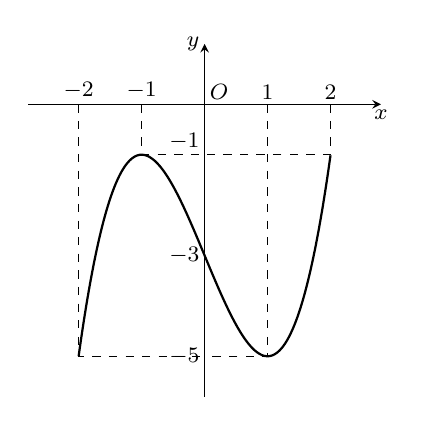
\begin{tikzpicture}[>=stealth,x=1cm,y=0.8cm,scale=0.8,font=\footnotesize]
		\draw[->] (-2.8,0) -- (2.8,0) node[below] {$x$};
		\draw[->] (0,-5.8) -- (0,1.2) node[left] {$y$};
		\draw (0,0) node[above right] {$O$};
		\draw[thick,smooth,samples=100] plot[domain=-2:2] (\x,{(\x)^3-3*(\x)-3});
		\draw[dashed] (-2,0) node[above] {$-2$} -- (-2,-5) -- (0,-5) node[left] {$-5$};
		\draw[dashed] (-1,0) node[above] {$-1$} -- (-1,-1) -- (0,-1) node[above left] {$-1$};
		\draw[dashed] (1,0) node[above] {$1$} -- (1,-5) -- (0,-5);
		\draw[dashed] (2,0) node[above] {$2$} -- (2,-1) -- (0,-1);
		\node[left] at (0,-3) {$-3$};
\end{tikzpicture}}
	\loigiai{
		Dựa vào đồ thị ta có $\max\limits_{[-2;2]} f(x) + \min\limits_{[-2;2]} f(x) = -1 + (-5) = -6$.
	}
\end{ex}

\begin{ex}%[2H2N2-3]%[Dự án C đề thi thử TN Môn Toán NH25-26 - Dot 4 - DuongPham]%[SGD-Hà Nội]%[GVPB - Đỗ Minh Vũ]
	Trong không gian với hệ trục tọa độ $Oxyz$, cho véc-tơ $\overrightarrow{u}= 3\overrightarrow{i} - 2\overrightarrow{j} + \overrightarrow{k}$. Tọa độ của véc-tơ $\overrightarrow{u}$ là
	\choice
	{\True $(3; -2; 1)$}
	{$(1; 3; -2)$}
	{$(3; 1; -2)$}
	{$(-2; 3; 1)$}
	\loigiai{
		Vectơ $\overrightarrow{u} = 3\overrightarrow{i} - 2\overrightarrow{j} + \overrightarrow{k}$ có tọa độ là $(3; -2; 1)$.
	}
\end{ex}

\begin{ex}%[1H8N7-2]%[Dự án C đề thi thử TN Môn Toán NH25-26 - Dot 4 - DuongPham]%[SGD-Hà Nội]%[GVPB - Đỗ Minh Vũ]
	Cho hình chóp $O.ABC$ có $OA$, $OB$, $OC$ đôi một vuông góc với nhau và $OA = a$, $OB = b$, $OC = c$. Thể tích của khối chóp $O.ABC$ bằng
	\choice
	{$\dfrac{abc}{3}$}
	{$abc$}
	{\True $\dfrac{abc}{6}$}
	{$\dfrac{abc}{2}$}
	\loigiai{
		Thể tích của khối chóp $O.ABC$ có ba cạnh $OA, OB, OC$ đôi một vuông góc là $$V = \dfrac{1}{6} \cdot OA \cdot OB \cdot OC = \dfrac{abc}{6}.$$
	}
\end{ex}

\begin{ex}%[2D4N3-3]%[Dự án C đề thi thử TN Môn Toán NH25-26 - Dot 4 - DuongPham]%[SGD-Hà Nội]%[GVPB - Đỗ Minh Vũ]
	Cho hàm số $y = f(x)$ liên tục và không âm trên đoạn $[0; 2]$. Thể tích khối tròn xoay sinh ra khi quay quanh trục $Ox$ hình phẳng giới hạn bởi đồ thị hàm số $y = f(x)$, trục hoành và hai đường thẳng $x = 0$, $x = 2$ là
	\choice
	{$\displaystyle\int_0^2 f(x) \mathrm{d}x$}
	{\True $\pi \displaystyle\int_0^2 [f(x)]^2 \mathrm{d}x$}
	{$\displaystyle\int_0^2 [f(x)]^2 \mathrm{d}x$}
	{$\pi \displaystyle\int_0^2 f(x) \mathrm{d}x$}
	\loigiai{
		Công thức tính thể tích khối tròn xoay khi quay hình phẳng giới hạn bởi đồ thị hàm số $y=f(x)$, trục hoành và hai đường thẳng $x=a$, $x=b$ quanh trục $Ox$ là $V = \pi \displaystyle\int_a^b [f(x)]^2 \mathrm{d}x$.
		Áp dụng với $a=0$, $b=2$, ta được $V = \pi \displaystyle\int_0^2 [f(x)]^2 \mathrm{d}x$.
	}
\end{ex}
\begin{ex}%[2D1N2-2]%[Dự án C đề thi thử TN Môn Toán NH25-26 - Dot 4 - DuongPham]%[SGD-Hà Nội]%[GVPB - Đỗ Minh Vũ]
	Cho hàm số $y = f(x)$ có đạo hàm trên $\mathbb{R}$ và có bảng xét dấu của $f'(x)$ như sau:
	\begin{center}
		\begin{center}
			
\begin{tikzpicture}
				\tkzTabInit[nocadre=true,lgt=2,espcl=2,deltacl=0.6]
				{$x$ /0.6,$f'(x)$ /0.6}
				{$-\infty$,$-3$,$1$,$2$,$+\infty$}
				\tkzTabLine{,-,$0$,+,$0$,+,$0$,-,}
			\end{tikzpicture}
		\end{center}
	\end{center}
	Số điểm cực trị của hàm số $y = f(x)$ là
	\choice 
	{$3$}
	{$1$}
	{\True $2$}
	{$0$}
	\loigiai{
		Hàm số có đạo hàm đổi dấu hai lần tại các điểm $x = -3$ (từ âm sang dương) và $x = 2$ (từ dương sang âm) nên hàm số có hai điểm cực trị. Tại điểm $x = 1$, đạo hàm bằng $0$ nhưng không đổi dấu nên đây không phải là điểm cực trị.
	}
\end{ex}

\begin{ex}%[2H2N1-2]%[Dự án C đề thi thử TN Môn Toán NH25-26 - Dot 4 - DuongPham]%[SGD-Hà Nội]%[GVPB - Đỗ Minh Vũ]
\immini[thm]{Cho hình hộp $ABCD.A'B'C'D'$ (tham khảo hình vẽ). Khi đó, tổng $\overrightarrow{AB} + \overrightarrow{AD} + \overrightarrow{DD'}$ bằng
	\choice 
	{$\overrightarrow{C'A}$}
	{\True $\overrightarrow{AC'}$}
	{$\overrightarrow{AD'}$}
	{$\overrightarrow{D'A}$}}
	{	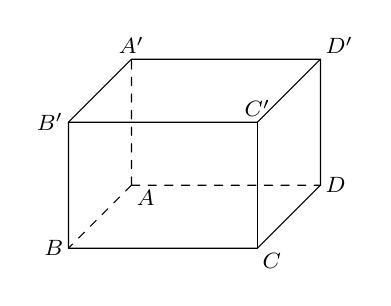
\begin{tikzpicture}[scale=0.8, font=\footnotesize, line join=round, line cap=round]
		\coordinate (B) at (0,0);
		\coordinate (C) at (3,0);
		\coordinate (A) at (1,1);
		\coordinate (D) at (4,1);
		\coordinate (Bp) at (0,2);
		\coordinate (Cp) at (3,2);
		\coordinate (Ap) at (1,3);
		\coordinate (Dp) at (4,3);
		\draw[dashed] (A) -- (B) (A) -- (D) (A) -- (Ap);
		\draw (B) -- (C) -- (D) -- (Dp) -- (Ap) -- (Bp) -- cycle;
		\draw (Bp) -- (Cp) -- (Dp);
		\draw (Cp) -- (C);
		\node[below right] at (A) {$A$};
		\node[left] at (B) {$B$};
		\node[below right] at (C) {$C$};
		\node[right] at (D) {$D$};
		\node[above] at (Ap) {$A'$};
		\node[left] at (Bp) {$B'$};
		\node[above] at (Cp) {$C'$};
		\node[above right] at (Dp) {$D'$};
\end{tikzpicture}}
	\loigiai{
		Ta có $\overrightarrow{AB} + \overrightarrow{AD} + \overrightarrow{DD'} = \overrightarrow{AB} + \overrightarrow{AD} + \overrightarrow{AA'} = \overrightarrow{AC'}$.
	}
\end{ex}

\begin{ex}%[2D4N1-2]%[Dự án C đề thi thử TN Môn Toán NH25-26 - Dot 4 - DuongPham]%[SGD-Hà Nội]%[GVPB - Đỗ Minh Vũ]
	Họ nguyên hàm của hàm số $f(x) = x^7$ là
	\choice
	{$8x^8 + C$}
	{$7x^6 + C$}
	{$\dfrac{x^7}{7} + C$}
	{\True $\dfrac{x^8}{8} + C$}
	\loigiai{
		Ta có $\displaystyle\int x^7 \mathrm{d}x = \dfrac{x^{7+1}}{7+1} + C = \dfrac{x^8}{8} + C$.
	}
\end{ex}

\begin{ex}%[1D1N4-2]%[Dự án C đề thi thử TN Môn Toán NH25-26 - Dot 4 - DuongPham]%[SGD-Hà Nội]%[GVPB - Đỗ Minh Vũ]
	Tập xác định của hàm số $y = \tan x$ là
	\choice
	{$\mathbb{R} \setminus \left\{\dfrac{\pi}{2} + k2\pi, k \in \mathbb{Z}\right\}$}
	{$\mathbb{R} \setminus \{k2\pi, k \in \mathbb{Z}\}$}
	{$\mathbb{R} \setminus \{k\pi, k \in \mathbb{Z}\}$}
	{\True $\mathbb{R} \setminus \left\{\dfrac{\pi}{2} + k\pi, k \in \mathbb{Z}\right\}$}
	\loigiai{
		Hàm số $y = \tan x$ xác định khi $\cos x \neq 0 \Leftrightarrow x \neq \dfrac{\pi}{2} + k\pi, k \in \mathbb{Z}$.\\
		Vậy tập xác định của hàm số là $\mathscr{D}=\mathbb{R} \setminus \left\{\dfrac{\pi}{2} + k\pi, k \in \mathbb{Z}\right\}$.
	}
\end{ex}
\TNTF

\begin{ex}%[Đề thi thử môn Toán SGD Hà Nội lần 1 năm học 2025-2026]%[Nguyễn Khánh Trọng - Đỗ Minh Vũ]%[1D9V2-4]
	Trong vòng chung kết của cuộc thi ĐƯỜNG ĐẾN VINH QUANG có $4$ thí sinh An, Bình, Toàn và Phương tham gia thi đấu. Sau khi An, Bình và Toàn hoàn thành phần thi cuối của mình, điểm số của ba bạn đạt được lần lượt là $180$ điểm, $200$ điểm và $170$ điểm. Bạn Phương là thí sinh cuối cùng bước vào phần thi cuối với điểm số hiện có là $190$ điểm. Tại phần thi cuối, mỗi thí sinh phải trả lời $3$ câu hỏi thuộc ba lĩnh vực: Tự nhiên, Xã hội và Tiếng Anh. Mỗi câu trả lời đúng được $20$ điểm, trả lời sai hoặc không trả lời bị trừ $10$ điểm. Thí sinh có quyền sử dụng \lq\lq Ngôi sao hy vọng\rq\rq\ tối đa một lần cho một trong ba câu hỏi, nếu trả lời đúng nhận được $40$ điểm, trả lời sai hoặc không trả lời bị trừ $20$ điểm. Biết xác suất Phương trả lời đúng câu hỏi thuộc lĩnh vực Tự nhiên, Xã hội và Tiếng Anh lần lượt là $0{,}7$; $0{,}4$ và $0{,}3$. Giả thiết rằng việc trả lời đúng mỗi câu hỏi không làm thay đổi xác suất trả lời đúng hoặc sai các câu hỏi còn lại.
	\choiceTF
	{\True Xác suất để Phương trả lời sai câu hỏi thuộc lĩnh vực Tự nhiên là $0{,}3$}
	{\True Xác suất để Phương trả lời đúng cả ba câu hỏi là $0{,}084$}
	{Xác suất để Phương trả lời đúng ít nhất một trong ba câu hỏi là $0{,}916$}
	{\True Nếu Phương chọn \lq\lq Ngôi sao hy vọng\rq\rq\ ở câu hỏi thuộc lĩnh vực Tự nhiên thì xác suất để Phương trở thành quán quân của cuộc thi này là $0{,}736$}
	\loigiai{
		\begin{itemchoice}
			\itemch Xác suất để Phương trả lời sai câu hỏi thuộc lĩnh vực Tự nhiên là $1-0{,}7=0{,}3$.
			\itemch Xác suất để Phương trả lời đúng cả ba câu hỏi là $0{,}7\cdot 0{,}4\cdot 0{,}3=0{,}084$.
			\itemch Xác suất để Phương trả lời đúng ít nhất một trong ba câu hỏi là $1-0{,}3\cdot 0{,}6\cdot 0{,}7=0{,}874$.
			\itemch Nếu Phương chọn \lq\lq Ngôi sao hy vọng\rq\rq\ ở câu hỏi thuộc lĩnh vực Tự nhiên.
			\begin{itemize}
				\item Trường hợp 1: Phương trả lời đúng câu Tự nhiên. Khi đó số điểm sẽ là $230$ điểm, vì vậy Phương sẽ thành quán quân cho dù trả lời sai hai câu kia.\\
				Xác suất của trường hợp này là $0{,}7$.
				\item Trường hợp 2: Phương trả lời sai câu tự nhiên. Khi đó số điểm sẽ là $170$ điểm, vì vậy muốn trở thành quán quân thì Phương phải trả lời đúng hai câu còn lại.\\
				Xác suất của trường hợp này là $0{,}3\cdot0{,}4\cdot0{,}3=0{,}036$.\\
				Do đó xác suất để Phương trở thành quán quân của cuộc thi này là $0{,}7+0{,}036=0{,}736$.
			\end{itemize}
		\end{itemchoice}
	}
\end{ex}

\begin{ex}%[Đề thi thử môn Toán SGD Hà Nội lần 1 năm học 2025-2026]%[Nguyễn Khánh Trọng - Đỗ Minh Vũ]%[2D4V2-6]
	Một người đang điều khiển ô tô chạy trên đường cao tốc. Khi cách trạm thu phí $1\,000$ m, tốc độ của ô tô là $90$ km/h. Sau $20$ giây, người điều khiển ô tô bắt đầu giảm tốc với tốc độ $v(t)=at+b$ (m/s), trong đó $t$ là thời gian tính bằng giây kể từ khi bắt đầu giảm tốc và $v(t) > 0$ với mọi $t\in[0;30]$. Sau $30$ giây kể từ khi bắt đầu giảm tốc, ô tô đến trạm thu phí.
	\choiceTF
	{\True Quãng đường từ vị trí ô tô bắt đầu giảm tốc đến trạm thu phí là $500$ m}
	{Giá trị của $b$ là $90$}
	{\True Giá trị của $a$ là $-\dfrac{5}{9}$}
	{\True Tốc độ tối đa cho phép của phương tiện khi qua trạm thu phí là $30$ km/h. Người điều khiển ô tô đó đã tuân thủ đúng tốc độ quy định khi đi qua trạm thu phí}
	\loigiai{
		\begin{itemchoice}
			\itemch Quãng đường từ vị trí ô tô bắt đầu giảm tốc đến trạm thu phí là $500$ m.\\
			Từ đầu đến khi ô tô bắt đầu giảm tốc, quãng đường đi được là $90\cdot\dfrac{20}{3\,600}=0{,}5$ km.\\
			Sau $20$ s quãng đường từ vị trí ô tô bắt đầu giảm tốc đến trạm thu phí là $1\,000-500=500$ (m).
			\itemch Vận tốc lúc bắt đầu giảm tốc là $90$ km/h $=25$ m/s. Giá trị của $b$ là $25$.
			\itemch Quãng đường đi được sau $30$ s lúc giảm phanh là $s=\displaystyle\int\limits_0^{30}\left(at+25\right)\mathrm{\,d}t=\dfrac{a}{2}\cdot30^2+750$.\\
			Theo đề bài ta được $\dfrac{a}{2}\cdot30^2+750=500\Leftrightarrow a=-\dfrac{5}{9}$.
			\itemch Vận tốc sau $30$ s là $v(30)=-\dfrac{5}{9}\cdot 30+25=\dfrac{25}{3}$ (m/s), suy ra vận tốc khi qua trạm thu phí là $30$ km/h.\\
			Tốc độ tối đa cho phép của phương tiện khi qua trạm thu phí là $30$ km/h.\\
			Người điều khiển ô tô đó đã tuân thủ đúng tốc độ quy định khi đi qua trạm thu phí.
		\end{itemchoice}
	}
\end{ex}

\begin{ex}%[Đề thi thử môn Toán SGD Hà Nội lần 1 năm học 2025-2026]%[Nguyễn Khánh Trọng - Đỗ Minh Vũ]%[2H5V1-5]
	Cho hình hộp chữ nhật $ABCD.A'B'C'D'$ có $AB=4$, $AD=3$ và $AA'=12$. Chọn hệ trục toạ độ $Oxyz$ với gốc $O$ trùng với điểm $A'$; các tia $A'B'$, $A'D'$, $A'A$ lần lượt trùng với các tia $Ox$, $Oy$, $Oz$ (tham khảo hình vẽ). Gọi $M$ là trung điểm của đoạn thẳng $AB$.
	\begin{center}
		\begin{tikzpicture}[scale=.7, font=\footnotesize, line join=round, line cap=round, >=stealth']
			\coordinate (A') at (0,0); % A' (gốc O)
			\coordinate (D') at (4,0); % B'
			\coordinate (B') at (-2,-1.5); % D'
			\coordinate (C') at ($(B')+(D')-(A')$);
			\coordinate (A) at ($(A')+(0,4)$);
			\coordinate (D) at ($(D')+(0,4)$);
			\coordinate (B) at ($(B')+(0,4)$);
			\coordinate (C) at ($(C')+(0,4)$);
			\coordinate (M) at ($(A)!0.5!(B)$);
			% Vẽ các cạnh thấy được
			\draw (B)--(C)--(D)--(A)--cycle;
			\draw (B)--(B')--(C')--(C);
			\draw (C')--(D')--(D);
			% Vẽ các cạnh khuất
			\draw[dashed] (A')--(B') (A')--(D') (A')--(A);
			% Vẽ hệ trục tọa độ
			\coordinate (y) at ($(A')!1.35!(D')$);
			\draw[->] (D')--(y) node[below]{$y$};
			\coordinate (x) at ($(A')!1.45!(B')$);
			\draw[->] (B')--(x) node[below]{$x$};
			\coordinate (z) at ($(A')!1.35!(A)$);
			\draw[->] (A)--(z) node[right]{$z$};
			% Ký hiệu điểm
			\foreach \t/\g in {A/45, B/180, C/-30, D/90, A'/45, B'/-90, C'/-45, D'/-90, M/120}{
				\fill (\t) circle (1pt) node[shift={(\g:8pt)}]{$\t$};
			}
		\end{tikzpicture}
	\end{center}
	\choiceTF
	{\True Toạ độ của điểm $D$ là $(0;3;12)$}
	{Toạ độ của vectơ $\overrightarrow{MD}$ là $(2;-3;0)$}
	{\True Một vectơ pháp tuyến của mặt phẳng $(MDC')$ có toạ độ là $(3;2;1)$}
	{Khoảng cách từ điểm $A'$ đến mặt phẳng $(MDC')$ lớn hơn $5$}
	\loigiai{
		\begin{itemchoice}
			\itemch Toạ độ của điểm $D$ là $(0;3;12)$.
			\itemch Ta có 
			$A(0;0;12)$, $B(4;0;12)$ $\Rightarrow M(2;0;12)$.\\
			$D(0;3;12)\Rightarrow\overrightarrow{MD}=(-2;3;0)$.
			\itemch Ta có $C'(4;3;0)$.\\
			Mặt phẳng $(MDC')$ có cặp vectơ chỉ phương là $\overrightarrow{MD}=(-2;3;0)$ và $\overrightarrow{MC'}=(2;3;-12)$.\\
			$\left[\overrightarrow{MD},\overrightarrow{MC'}\right]=(-36;-24;-12)$.\\
			Một vectơ pháp tuyến của mặt phẳng $\left(MD{C}'\right)$ là
			$\overrightarrow{n}=-\dfrac{1}{12}\cdot\left[\overrightarrow{MD},\overrightarrow{MC'}\right]=(3;2;1)$.
			\itemch 
			Mặt phẳng $(MDC')$ đi qua điểm $C'\left(4;3;0\right)$ và có một vectơ pháp tuyến là $\overrightarrow{n}(3;2;1)$. Suy ra
			$(MDC')$ có phương trình $$3(x-4)+2(y-3)+1(z-0)=0\Leftrightarrow 3x+2y+z-18=0.$$
			Khoảng cách từ điểm $A'(0;0;0)$ đến mặt phẳng $(MDC')$ là $$\mathrm{d}(A',(MDC'))=\dfrac{\left| 3\cdot0+2\cdot0+0-18\right|}{\sqrt{3^2+2^2+1^2}}=\dfrac{18}{\sqrt{14}}\approx 4{,}81<5.$$
		\end{itemchoice}
	}
\end{ex}

\begin{ex}%[Đề thi thử môn Toán SGD Hà Nội lần 1 năm học 2025-2026]%[Nguyễn Khánh Trọng - Đỗ Minh Vũ]%[2D1V5-1]
	Cho hàm số $y=\dfrac{ax^2+bx+c}{x+d}$ ($a\ne 0$) có đồ thị là đường cong $(C)$. Các đường thẳng $d_1$, $d_2$ lần lượt là tiệm cận đứng và tiệm cận xiên của đường cong $(C)$ như hình vẽ.
	\begin{center}
		\begin{tikzpicture}[line join=round,line cap=round,>=stealth,scale=0.6,font=\footnotesize]
			\tikzset{every node/.style={outer sep=-0.5mm}}
			\def \xmin{-6} \def \xmax{6}
			\def \ymin{-6.5} \def \ymax{4.5}
			\def \fx{((\x)^2+\x-6)/(\x+1)}
			\def \gx{\x}
			\draw[->] (\xmin,0)--(\xmax,0) node[below left] {\normalsize$x$};
			\draw[->] (0,\ymin)--(0,\ymax) node[below left] {\normalsize$y$};
			\draw (0,0) node[below right] {$O$};
			\draw (-1,\ymin)--(-1,\ymax);
			\fill (-1,0) circle (1.25pt) node[above left] {$-1$};
			\fill (0,-1) circle (1.25pt) node[right] {$-1$};
			\fill (2,0) circle (1.25pt) node[above left] {$2$};
			\draw[dashed,thin](-1,0)--(-1,-1)--(0,-1);
			\draw (-1,2) node[left]{$d_1$};
			\draw (2.8,3) node[left]{$d_2$};
			\draw (4.2,3) node[right]{$(C)$};
			\begin{scope}
				\clip (\xmin+0.01,\ymin+0.01) rectangle (\xmax-0.01,\ymax-0.01);
				\draw[samples=150,domain=\xmin+0.01:-1-0.1,smooth,variable=\x] plot (\x,{\fx});
				\draw[samples=150,domain=-1+0.1:\xmax-0.01,smooth,variable=\x] plot (\x,{\fx});
				\draw[samples=350,domain=\xmin+0.1:\xmax-0.01,smooth,variable=\x] plot (\x,{\gx});
			\end{scope}
		\end{tikzpicture}
	\end{center}
	\choiceTF
	{Đồ thị $(C)$ đi qua điểm có toạ độ $(0;2)$}
	{\True Đồ thị $(C)$ có tiệm cận đứng là đường thẳng $x=-1$}
	{\True Đồ thị $(C)$ có tiệm cận xiên là đường thẳng $y=x$}
	{\True Giá trị của tổng $a+b+c+d$ là một số âm}
	\loigiai{
		\begin{itemchoice}
			\itemch Đồ thị $(C)$ có điểm chung với trục $Oy$ và điểm chung này có tung độ âm.
			\itemch Đồ thị $(C)$ có tiệm cận đứng là đường thẳng $x=-1$.
			\itemch Đồ thị $(C)$ có tiệm cận xiên là đường thẳng $y=x$.
			\itemch Ta có
			\begin{itemize}
				\item Đồ thị $(C)$ có tiệm cận đứng là đường thẳng $x=-1$ nên $d=1 \Rightarrow y=\dfrac{ax^2+bx+c}{x+1}$.
				\item Đồ thị $(C)$ đi qua điểm $(2;0)$ nên $0=\dfrac{a\cdot2^2+b\cdot2+c}{2+1}\Rightarrow 4a+2b+c=0$ (1).\\
				\item $y=\dfrac{ax^2+bx+c}{x+1}=ax+b-a+\dfrac{a-b+c}{x+1}$.\\
				Suy ra đồ thị hàm số $y=\dfrac{ax^2+bx+c}{x+1}$ có đường tiệm cận xiên là đường thẳng $y=ax+b-a$.\\
				Dựa vào hình vẽ thì đồ thị hàm số $y=\dfrac{ax^2+bx+c}{x+1}$ có tiệm cận xiên là đường thẳng $y=x$ nên $\heva{& a=1\\ & b-a=0}\Leftrightarrow a=b=1$ (2).\\
				Từ (1) và (2) $\Rightarrow a=b=1$, $c=-6$.\\
				Suy ra $a+b+c+d=1+1-6+1=-3$.
			\end{itemize}
			Vậy, $a+b+c+d$ là một số âm.
		\end{itemchoice}
	}
\end{ex}
\TNSA
\begin{ex}%%[Đề thi thử môn Toán SGD Hà Nội lần 1 năm học 2025-2026]%[Hiep Quang Nguyen - Đỗ Minh Vũ]%[0H4V3-2]
	Cho hình vuông $ABCD$ có độ dài cạnh bằng $1$. Cung $AC$ là một phần tư đường tròn tâm $D$, bán kính $DA$ (tham khảo hình vẽ). Giả sử $P$ là điểm thay đổi trên cung $AC$ ($P$ khác $A$ và $C$). Tiếp tuyến tại điểm $P$ của cung $AC$ cắt các đoạn thẳng $AB$, $BC$ theo thứ tự tại các điểm $M$, $N$.
	\begin{center}
		\begin{tikzpicture}[scale=3, font=\footnotesize, line join=round, line cap=round, >=stealth]
			\coordinate (D) at (0,0);
			\coordinate (C) at (1,0);
			\coordinate (B) at (1,1);
			\coordinate (A) at (0,1);
			\draw (A)--(B)--(C)--(D)--cycle;
			\draw (C) arc (0:90:1);
			\pgfmathsetmacro{\ang}{50}
			\coordinate (P) at ({cos(\ang)},{sin(\ang)});
			\coordinate (M) at ({(1-sin(\ang))/cos(\ang)},1);
			\coordinate (N) at (1,{(1-cos(\ang))/sin(\ang)});
			
			\fill[pattern=north east lines, opacity=0.5] (M)--(B)--(N)--cycle;
			\draw (M)--(N);
			
			\draw[fill=black] (A) circle (0.5pt) node[above left] {$A$};
			\draw[fill=black] (B) circle (0.5pt) node[above right] {$B$};
			\draw[fill=black] (C) circle (0.5pt) node[below right] {$C$};
			\draw[fill=black] (D) circle (0.5pt) node[below left] {$D$};
			\draw[fill=black] (M) circle (0.5pt) node[above] {$M$};
			\draw[fill=black] (N) circle (0.5pt) node[right] {$N$};
			\draw[fill=black] (P) circle (0.5pt) node[below left] {$P$};
		\end{tikzpicture}
	\end{center}
	Diện tích lớn nhất của tam giác $BMN$ bằng bao nhiêu (kết quả làm tròn đến hàng phần trăm)?
	\shortans[oly]{$0{,}17$}
	\loigiai{
		Đặt $AM = x$ và $CN = y$.\\
		Do $AM$, $PM$ và $CN$, $PN$ là các tiếp tuyến cắt nhau nên $MP = AM = x$ và $PN = CN = y$.\\
		Tam giác $BMN$ vuông tại $B$ nên \allowdisplaybreaks
		\begin{eqnarray*}
			&&MN^2 = MB^2 + BN^2 \\
			&\Leftrightarrow& (x+y)^2 = (1-x)^2 + (1-y)^2\\
			&\Leftrightarrow& xy + x + y = 1 \\
			&\Leftrightarrow& (x+1)(y+1) = 2.
		\end{eqnarray*}
		Ta có $S_{BMN}=\dfrac{1}{2} BM \cdot BN=\dfrac{1}{2}(1-x)(1-y)=\dfrac{1}{2}(1-x-y+xy)=xy$.\\
		Áp dụng bất đẳng thức Cauchy-Schwarz:
		\[\sqrt{x}\sqrt{y}+1 \cdot 1 \le \sqrt{(x+1)(y+1)} \Rightarrow \sqrt{x}\sqrt{y} \le \sqrt{(x+1)(y+1)}-1=\sqrt{2}-1 \Leftrightarrow xy \le \left(\sqrt{2}-1\right)^2.\]
		Đẳng thức xảy ra khi và chỉ khi $\heva{& \sqrt{x}=\sqrt{y} \\ & (x+1)(y+1)=2} \Leftrightarrow x=y=\sqrt{2}-1$.\\
		Vậy diện tích lớn nhất của tam giác $BMN$ là $\left(\sqrt{2}-1\right)^2=3-2\sqrt{2} \approx 0{,}17$.
	}
\end{ex}
\begin{ex}%%[Đề thi thử môn Toán SGD Hà Nội lần 1 năm học 2025-2026]%[Hiep Quang Nguyen - Đỗ Minh Vũ]%[1D9C2-4]
	Người ta trang trí một bảng ô vuông $4 \times 4$ (như Hình 1) bởi các ngôi sao và các bông hoa giống nhau. Mỗi ô vuông nhỏ được dán một ngôi sao hoặc một bông hoa, sao cho trong mỗi hàng hoặc mỗi cột của bảng ô vuông đều có $2$ ngôi sao và $2$ bông hoa (tham khảo một cách dán trong Hình 2).
	\begin{center}
		\begin{tikzpicture}[scale=0.6, font=\footnotesize, line join=round, line cap=round, thick]
			% Hình 1
			\draw (0,0) grid (4,4);
			\node at (2,-0.5){\textbf{Hình 1}};
			
			% Hình 2
			\begin{scope}[xshift=7cm]
				\draw (0,0) grid (4,4);
				\node at (2,-0.5){\textbf{Hình 2}};
				\def\s{$\bigstar$}
				\def\h{\begin{tikzpicture}[scale=0.08, baseline=-0.5ex] 
						\draw (0,1) circle (1);
						\draw (0,-1) circle (1);
						\draw (1,0) circle (1);
						\draw (-1,0) circle (1);
						\draw (0,0) circle (0.4);
				\end{tikzpicture}}
				
				% Row 4
				\node at (0.5, 3.5){\s};\node at (1.5, 3.5){\h};\node at (2.5, 3.5){\s};\node at (3.5, 3.5){\h};
				% Row 3
				\node at (0.5, 2.5){\h};\node at (1.5, 2.5){\s};\node at (2.5, 2.5){\h};\node at (3.5, 2.5){\s};
				% Row 2
				\node at (0.5, 1.5){\s};\node at (1.5, 1.5){\h};\node at (2.5, 1.5){\s};\node at (3.5, 1.5){\h};
				% Row 1
				\node at (0.5, 0.5){\h};\node at (1.5, 0.5){\s};\node at (2.5, 0.5){\h};\node at (3.5, 0.5){\s};
			\end{scope}
		\end{tikzpicture}
	\end{center}
	Có tất cả bao nhiêu cách trang trí bảng ô vuông thỏa mãn yêu cầu trên?
	\shortans[oly]{$2502$}
	\loigiai{
		\begin{enumerate}[\textbf{Cách} 1:]
			\item 
			Đặt mỗi ngôi sao là $1$ điểm và mỗi bông hoa là $0$ điểm, khi đó bài toán trở thành xếp các số vào bảng sao cho tổng mỗi hàng hoặc mỗi cột bằng $2$.\\
			Gọi $A$ là biến cố: \lq\lq Tổng mỗi hàng bằng $2$\rq\rq\, và $B$ là biến cố: \lq\lq Tổng mỗi cột là $2$\rq\rq\,.\\
			Ta có $n(A)=n(B)=\left(C_4^2\right)^4=1296$.\\
			Khi đó ta cần tìm số phần tử của tập $A \cup B$.\\
			Ta xét biến cố $A \cap B$: \lq\lq Tổng mỗi hàng và cột bằng $2$\rq\rq\,.\\
			Ta xét các trường hợp hàng ngang thỏa mãn là
			\begin{itemize}
				\item Loại $I$: $(1;1;0;0)$, $(0;0;1;1)$.
				\item Loại $II$: $(0;1;1;0)$, $(1;0;0;1)$.
				\item Loại $III$: $(1;0;1;0)$, $(0;1;0;1)$.
			\end{itemize}
			\textbf{Trường hợp 1:} Nếu cộng mỗi cặp cùng loại ta thấy rằng tổng các cột sẽ là $1$ nên ta sẽ dùng $2$ hàng loại $I$ là $(1;1;0;0)$, $(0;0;1;1)$.\\
			Xếp $2$ hàng $(1;1;0;0)$ vào $2$ trong $4$ hàng có $C_4^2$ cách và xếp $2$ hàng $(0;0;1;1)$ vào $2$ hàng còn lại có $1$ cách.\\
			Tương tự với loại $II$ và $III$, trường hợp này ta có $C_4^2 \cdot 1 \cdot 3=18$ cách.\\[4pt]
			\textbf{Trường hợp 2:} Nếu cộng $4$ cặp khác nhau ở $2$ loại ta thấy rằng tổng các cột sẽ là $2$ nên ta sẽ dùng $4$ hàng từ $2$ loại.\\
			Chọn $2$ loại từ $3$ loại có $C_3^2$ cách.\\
			Sau khi chọn được $2$ loại, ta sẽ có $4$ hàng. Do các hàng đôi một khác nhau nên hoán vị hàng có $4!$ cách.\\
			Trường hợp này ta có $C_3^2 \cdot 4!=72$.\\
			Vậy các trường hợp của biến cố $A \cap B$ là $18+72=90$.\\
			Khi đó, $n(A \cup B)=n(A)+n(B)-n(A \cap B)=1296+1296-90=2502$.
			\item 
			Đặt mỗi ngôi sao biểu diễn bởi số $1$ và mỗi bông hoa biểu diễn bởi số $0$.\\
			Ta sẽ xếp lần lượt từng hàng:\\
			Hàng $I$: Chọn vị trí cho $2$ số $1$ có $C_4^2$ cách và $2$ số $0$ vào hai vị trí còn lại có $1$ cách, nên hàng $I$ có $6$ cách xếp.\\
			Hàng $II$ và $III$ ta sẽ xét ba trường hợp:\\[4pt]
			\textbf{Trường hợp 1:}
			\begin{center}
				\begin{tabular}{|c|c|c|c|}
					\hline
					$1$ & $0$ & $0$ & $1$ \\ \hline
					$1$ & $0$ & $0$ & $1$ \\ \hline
					$0$ & $1$ & $1$ & $0$ \\ \hline
					& & & \\ \hline
				\end{tabular}
			\end{center}
			Hàng thứ $II$ giống hàng $I$ sẽ có $1$ cách xếp.\\
			Hàng thứ $III$ do đã có $2$ cột đủ số $1$ nên hàng thứ $III$ chỉ có $1$ cách xếp vào $2$ cột còn lại.\\[4pt]
			\textbf{Trường hợp 2:}
			\begin{center}
				\begin{tabular}{|c|c|c|c|}
					\hline
					$1$ & $0$ & $0$ & $1$ \\ \hline
					$0$ & $1$ & $0$ & $1$ \\ \hline
					$1$ & $0$ & $1$ & $0$ \\ \hline
					& & & \\ \hline
				\end{tabular}
			\end{center}
			Hàng thứ $II$ có vị trí $1$ số $1$ giống với vị trí của $1$ số $1$ trên hàng $I$ và số $1$ còn lại khác vị trí số còn lại của hàng $I$, lúc này hàng $II$ sẽ có $2 \cdot 2=4$ cách xếp.\\
			Hàng thứ $III$ phải có $1$ số $1$ vào cột chưa có số $1$ nên có $1$ cách. Số $1$ còn lại vào $2$ cột chỉ có $1$ số $1$ sẽ có $2$ cách, lúc này hàng $III$ sẽ có $1 \cdot 2=2$ cách xếp.\\[4pt]
			\textbf{Trường hợp 3:}
			\begin{center}
				\begin{tabular}{|c|c|c|c|}
					\hline
					$1$ & $0$ & $0$ & $1$ \\ \hline
					$0$ & $1$ & $1$ & $0$ \\ \hline
					$1$ & $0$ & $1$ & $0$ \\ \hline
					& & & \\ \hline
				\end{tabular}
			\end{center}
			Hàng thứ $II$ không có vị trí số $1$ trùng vị trí số $1$ ở hàng $I$ nên có $1$ cách xếp.\\
			Do mỗi cột chỉ mới có $1$ số $1$ nên hàng thứ $III$ xếp bất kì đều được nên hàng $III$ có $6$ cách xếp.\\[4pt]
			Hàng $IV$:\\
			Hàng thứ $IV$ sẽ điều chỉnh để thỏa mãn theo hàng $I$, $II$ và $III$ nên chỉ có $1$ cách xếp.\\
			Vậy có tất cả $6 \cdot (1 \cdot 1+4 \cdot 2+1 \cdot 6) \cdot 1=90$ cách xếp thỏa mãn điều kiện $A \cap B$.\\
			Từ đó ta suy ra $n(A \cup B)=n(A)+n(B)-n(A \cap B)=1296+1296-90=2502$.		
		\end{enumerate}
	}
\end{ex}

\begin{ex}%%[Đề thi thử môn Toán SGD Hà Nội lần 1 năm học 2025-2026]%[Hiep Quang Nguyen - Đỗ Minh Vũ]%[1D6V3-5]
	Sau khi một loại thuốc kháng sinh được tiêm vào cơ thể thì nồng độ của thuốc trong máu sẽ giảm dần theo thời gian do quá trình chuyển hóa. Nồng độ thuốc trong máu sau $t$ giờ kể từ khi tiêm được mô hình hóa bởi công thức $C(t)=C_0\mathrm{e}^{-rt}$ (mg/lít). Trong đó:
	\begin{itemize}
		\item $C_0$ là nồng độ thuốc trong máu ngay sau khi tiêm.
		\item $r$ là hằng số dương đo tốc độ phân hủy của thuốc.
		\item $\mathrm{e} \approx 2{,}718$.
	\end{itemize}
	Biết rằng ngay sau khi tiêm, nồng độ thuốc trong máu là $15$ mg/lít và sau đó $4$ giờ nồng độ thuốc giảm còn $10$ mg/lít. Để đạt hiệu quả điều trị, bác sĩ sẽ tiêm lại một liều mới khi nồng độ thuốc trong máu của bệnh nhân giảm xuống và còn ít nhất $6$ mg/lít. Theo mô hình trên, để đạt hiệu quả điều trị thì khoảng thời gian nhiều nhất giữa hai lần tiêm thuốc là bao nhiêu giờ? (kết quả làm tròn đến hàng đơn vị).
	\shortans[oly]{$9$}
	\loigiai{
		Ngay sau khi tiêm, nồng độ thuốc trong máu là $15$ mg/lít nên ta có
		\[C(0)=C_0\mathrm{e}^{-r\cdot 0}=15 \Leftrightarrow C_0=15.\]
		Sau đó $4$ giờ nồng độ thuốc giảm còn $10$ mg/lít nên ta có
		\[C(4)=15\mathrm{e}^{-r\cdot 4}=10 \Leftrightarrow \mathrm{e}^{-4r}=\dfrac{2}{3} \Leftrightarrow -4r = \ln\dfrac{2}{3} \Leftrightarrow r=\dfrac{1}{4}\ln\dfrac{3}{2}.\]
		Để đạt hiệu quả điều trị, nồng độ thuốc trong máu còn ít nhất $6$ mg/lít
		\[C(t)=15\mathrm{e}^{-\tfrac{1}{4}\ln\left(\tfrac{3}{2}\right)\cdot t} \ge 6 \Leftrightarrow -\dfrac{1}{4}\ln\left(\dfrac{3}{2}\right)\cdot t \ge \ln\dfrac{6}{15} \Leftrightarrow t \le \dfrac{\ln\tfrac{6}{15}}{-\tfrac{1}{4}\ln\left(\tfrac{3}{2}\right)} \approx 9.\]
		Vậy để đạt hiệu quả điều trị thì khoảng thời gian nhiều nhất giữa hai lần tiêm thuốc là $9$ giờ.
	}
\end{ex}

\begin{ex}%[Đề thi thử môn Toán SGD Hà Nội lần 1 năm học 2025-2026]%[Hiep Quang Nguyen - Đỗ Minh Vũ]%%[1D2V2-7]
	Anh Tú vay ngân hàng $300$ triệu đồng để mua xe ô tô với lãi suất cố định $7{,}2\%$/năm theo hình thức trả góp hằng tháng, trong thời hạn $12$ tháng (ứng với $12$ kì trả nợ). Trong thời hạn đó, cuối mỗi kì trả nợ, anh Tú phải trả $25$ triệu đồng tiền gốc (ứng với $300$ triệu đồng chia đều cho $12$ tháng) và một khoản tiền lãi được tính theo số tiền dư nợ còn lại. Sau $12$ tháng, tổng số tiền lãi anh Tú phải trả ngân hàng là bao nhiêu triệu đồng (kết quả làm tròn đến hàng phần mười)?
	\shortans[oly]{$11{,}7$}
	\loigiai{
		Số tiền còn nợ mỗi tháng tạo thành cấp số cộng với số hạng đầu $u_1=300$, công sai $d=-25$ và số số hạng $n=12$. Suy ra tổng số tiền dư nợ trong $12$ tháng là
		\[S_n=\dfrac{n\left[2u_1+(n-1)d\right]}{2}=\dfrac{12\left[2 \cdot 300+(12-1) \cdot (-25)\right]}{2}=1\,950.\]
		Lãi suất tương ứng theo tháng là $\dfrac{7{,}2\%}{12}=0{,}6\%$.\\
		Tổng số tiền lãi anh Tú phải trả là $1\,950 \cdot 0{,}6\%=11{,}7$ (triệu đồng).
	}
\end{ex}

\begin{ex}%[2D4V3-1]
	Trong lưới ô vuông có hai đường parabol như hình vẽ. Biết rằng mỗi ô vuông nhỏ có cạnh bằng $1$ cm. Diện tích của hình phẳng trong lưới ô vuông được giới hạn bởi hai đường parabol (phần gạch chéo) bằng bao nhiêu centimet vuông (kết quả làm tròn đến hàng phần trăm)?
	\begin{center}
		\begin{tikzpicture}[scale=0.5, font=\footnotesize, line join=round, line cap=round, >=stealth]
			\clip (-4.01,0) rectangle (4.01,8);
			\draw[step=1cm,gray,dashed,very thin] (-5,-1) grid (5,9);
			\draw[thick] (-4,0) rectangle (4,8);
			\draw[domain=-4.2:4.2, smooth, variable=\x] plot ({\x}, {0.5*\x*\x});
			\draw[domain=-4.5:4.5, smooth, variable=\x] plot ({\x}, {11/48*\x*\x - 1/8*\x + 11/6});
			\clip (-4,0) rectangle (5,9);
			\fill[pattern=north east lines] plot[domain=-4:4] ({\x}, {0.5*\x*\x}) -- plot[domain=4:-4] ({\x}, {11/48*\x*\x - 1/8*\x + 11/6}) -- cycle;
		\end{tikzpicture}
	\end{center}
	\shortans[oly]{$9{,}76$}
	\loigiai{
		Chọn hệ trục tọa độ $Oxy$ như hình vẽ.
		\begin{center}
			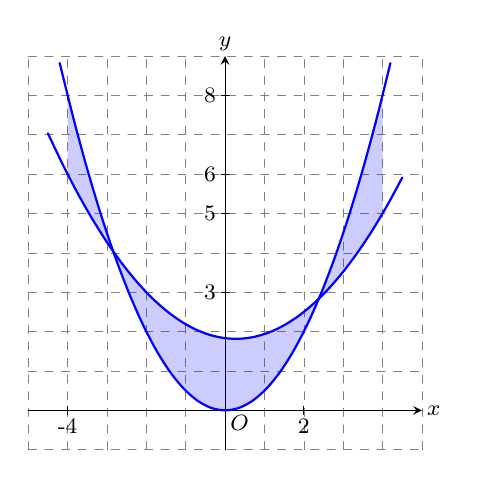
\begin{tikzpicture}[scale=0.5, font=\footnotesize, line join=round, line cap=round, >=stealth]
				\draw[step=1cm,gray,dashed,very thin] (-5,-1) grid (5,9);
				\draw[->] (-5,0) -- (5,0) node[right] {$x$};
				\draw[->] (0,-1) -- (0,9) node[above] {$y$};
				\draw (0,0) node[below right] {$O$};
				\foreach \x in {-4,2} \draw (\x,0.1) -- (\x,-0.1) node[below] {\x};
				\foreach \y in {3,5,6,8} \draw (0.1,\y) -- (-0.1,\y) node[left] {\y};
				\draw[domain=-4.2:4.2, smooth, variable=\x, blue, thick] plot ({\x}, {0.5*\x*\x});
				\draw[domain=-4.5:4.5, smooth, variable=\x, blue, thick] plot ({\x}, {11/48*\x*\x - 1/8*\x + 11/6});
				\clip (-5,-1) rectangle (5,9);
				\fill[blue, opacity=0.2] plot[domain=-4:4] ({\x}, {0.5*\x*\x}) -- plot[domain=4:-4] ({\x}, {11/48*\x*\x - 1/8*\x + 11/6}) -- cycle;
			\end{tikzpicture}
		\end{center}
		Gọi $(P_1) \colon y = ax^2 + bx + c$ với $a>0$ đi qua các điểm $A(-4;8)$, $O(0;0)$, $B(4;8)$ nên ta có
		\[\heva{& 16a - 4b + c = 8 \\ & 16a + 4b + c = 8 \\ & c = 0} \Rightarrow \heva{& a = \dfrac{1}{2} \\ & b = c = 0.}\]
		Suy ra $(P_1) \colon y = \dfrac{1}{2}x^2$.\\
		Gọi $(P_2) \colon y = mx^2 + nx + p$ với $m>0$ đi qua các điểm $D(-4;6)$, $E(-2;3)$, $F(4;5)$ nên ta có
		\[\heva{& 16m - 4n + p = 6 \\ & 16m + 4n + p = 5 \\ & 4m - 2n + p = 3} \Rightarrow \heva{& m = \dfrac{11}{48} \\ & n = -\dfrac{1}{8} \\ & p = \dfrac{11}{6}.}\]
		Suy ra $(P_2) \colon y = \dfrac{11}{48}x^2 - \dfrac{1}{8}x + \dfrac{11}{6}$.\\
		Diện tích của hình phẳng trong lưới ô vuông được giới hạn bởi hai đường parabol
		\[S = \displaystyle\int\limits_{-4}^{4} \left| \dfrac{1}{2}x^2 - \left(\dfrac{11}{48}x^2 - \dfrac{1}{8}x + \dfrac{11}{6}\right) \right| \, \mathrm{d}x \approx 9{,}76 \text{ (cm}^2\text{)}.\]
	}
\end{ex}

\begin{ex}%[Đề thi thử môn Toán SGD Hà Nội lần 1 năm học 2025-2026]%[Hiep Quang Nguyen - Đỗ Minh Vũ]%%[1H8V6-2]
	Cho hình chóp tứ giác $S.ABCD$ có đáy $ABCD$ là hình vuông cạnh bằng $2$. Biết rằng $SA$ vuông góc với mặt phẳng $(ABCD)$ và $SA = \sqrt{6}$ (tham khảo hình vẽ). Góc phẳng nhị diện $[S, BD, C]$ có số đo bằng bao nhiêu độ?
	\begin{center}
		\begin{tikzpicture}[scale=1, font=\footnotesize, line join=round, line cap=round, >=stealth]
			\coordinate (A) at (0,0);
			\coordinate (B) at (-1.5,-1);
			\coordinate (D) at (3,0);
			\coordinate (C) at (1.5,-1);
			\coordinate (S) at (0,3.5);
			\coordinate (I) at ($(A)!0.5!(C)$);
			
			\draw[dashed] (A)--(B) (A)--(D) (S)--(A) (A)--(C) (B)--(D) (S)--(I);
			\draw (S)--(B)--(C)--(D)--cycle (S)--(C);
			\draw[dashed] (0.2,0) -- (0.2,0.2) -- (0,0.2);
			
			\foreach \p/\pos in {S/above, A/above left, B/below left, C/below right, D/right, I/below}
			\fill (\p) circle (1.5pt) node[\pos] {$\p$};
		\end{tikzpicture}
	\end{center}
	\shortans[oly]{$120$}
	\loigiai{
		Gọi $I$ là tâm hình vuông $ABCD$.\\
		Ta có $\heva{& BD \perp AC \\ & BD \perp SA} \Rightarrow BD \perp (SAC) \Rightarrow BD \perp AI, BD \perp SI$.\\
		Suy ra $[S, BD, C] = \widehat{SIC} = 180^\circ - \widehat{SIA}$.\\
		Trong $\triangle SAI$ vuông tại $A$ ta có $SA = \sqrt{6}$, $AI = \dfrac{AC}{2} = \dfrac{2\sqrt{2}}{2} = \sqrt{2}$.\\
		Khi đó $\tan \widehat{SIA} = \dfrac{SA}{AI} = \dfrac{\sqrt{6}}{\sqrt{2}} = \sqrt{3} \Rightarrow \widehat{SIA} = 60^\circ$.\\
		Vậy $[S, BD, C] = \widehat{SIC} = 180^\circ - \widehat{SIA} = 120^\circ$.
	}
\end{ex}
